\documentclass[../EngineeringJournal_CDavis.tex]{subfiles}

\begin{document}

%%%%%%%%%%%%%%%%%%%%%%%%%%%%%%%%%%%%%%%%%%%%%%%%%%%%%
%%%%%%%%%%%%%%%%%%%%%%%%%%%%%%%%%%%%%%%%%%%%%%%%%%%%%

\chapter[Configuring Vlans and Trunks]{Configuring Vlans\linebreak[1] and
Trunks \hspace*{\fill March 4, 2020}}
\noindent\textbf{{Packet Tracer Lab 13} \hspace*{\fill}{\textbf{CIT 167}}}\linebreak[1]
{{Spring 2020} \hspace*{\fill}{Chaz Davis}}                             
%===================================
%===================================


\hspace{0.2cm}
\begin{tcolorbox}[width=6.3in]
\scriptsize 
vlans and trunks
  \begin{outline}
    \1 blah blah blah
  \end{outline}
\end{tcolorbox}
\hspace{0.2cm}
\normalsize  
  
\clearpage

%===================================
\mysection{\textbf{Part 1: Configuration}}

I set up the configurations for each pc on the network. I then copied and
pasted the commands from the handout for each of the switches.
The network is all up and running.

\begin{figure}[!h]
  \centering
  {\label{run13}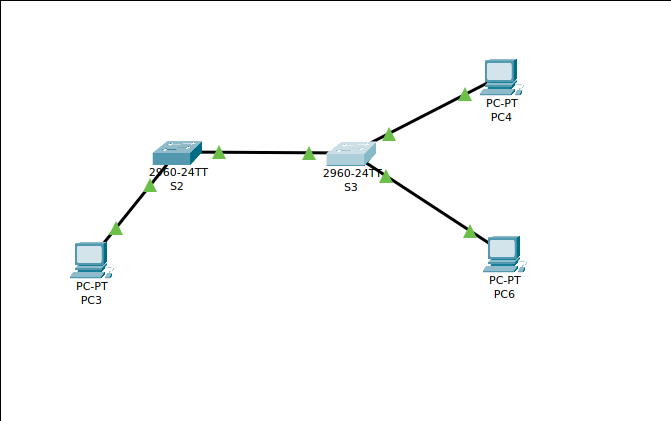
\includegraphics[width=.45\linewidth]{Figures/2020-03-08-183211_671x421_scrot.png}}
  \caption{The Network Up and Running}
\end{figure}


%===================================

\end{document}
